\documentclass[aspectratio=169,11pt]{beamer}

\usetheme{Madrid}
\usecolortheme{default}
\setbeamertemplate{navigation symbols}{}
\setbeamertemplate{footline}[frame number]

\usepackage{amsmath,amssymb}
\usepackage{graphicx}
\usepackage{tikz}
\usetikzlibrary{positioning,calc}
\usetikzlibrary{arrows.meta,decorations.pathmorphing}

\definecolor{RamRed}{RGB}{190,40,45}
\definecolor{RamBlue}{RGB}{30,90,180}
\definecolor{SoftGray}{RGB}{245,245,245}
\definecolor{DarkGray}{RGB}{70,70,70}
\definecolor{MapGreen}{RGB}{48,150,95}
\definecolor{MapGold}{RGB}{235,180,45}

\setbeamercolor{title}{fg=DarkGray}
\setbeamercolor{frametitle}{fg=white,bg=RamBlue}
\setbeamercolor{structure}{fg=RamBlue}

\tikzset{
  v/.style={circle,draw=black,fill=white,inner sep=1.8pt},
  edge/.style={draw=RamBlue,line width=1.25pt},
  topic/.style={draw=black!30,fill=SoftGray,rounded corners=5pt,inner sep=7pt,
    text width=5.8cm,minimum height=1.65cm,align=left},
}


\usepackage{booktabs}
\tikzset{dot/.style={circle,fill=black,inner sep=2pt}, lab/.style={circle,draw=black,fill=white,inner sep=2pt,minimum size=6mm,font=\small},selected/.style={draw=RamRed,line width=2pt}}

\newcommand{\Def}[2]{\begin{block}{#1}#2\end{block}}
\newcommand{\Thm}[2]{\begin{block}{#1}#2\end{block}}
\renewcommand{\Proof}[1]{\begin{block}{Proof}\normalsize #1\end{block}}
\newcommand{\Question}[1]{\begin{block}{Question}#1\end{block}}
\renewcommand{\Example}[1]{\begin{block}{Example}#1\end{block}}
\newcommand{\fall}[2]{#1^{\underline{#2}}}
\newcommand{\rise}[2]{#1^{\overline{#2}}}
\newcommand{\stir}[2]{\left\{\begin{matrix}#1\\#2\end{matrix}\right\}}
\newcommand{\cyc}[2]{\left[\begin{matrix}#1\\#2\end{matrix}\right]}
\newcommand{\eul}[2]{\left\langle\begin{matrix}#1\\#2\end{matrix}\right\rangle}
\newcommand{\coef}[2]{[#1^{#2}]}
\newcommand{\gap}{\par\medskip}

\title{Binomial Coefficients}
\author{Jeremy Quastel}\date{}\begin{document}
\begin{frame}[plain]\begin{center}{\Huge\bfseries Binomial Coefficients}\par\vspace{.25cm}{\Large Section 2.2}\par\vspace{.15cm}{\large Harris--Hirst--Mossinghoff, \emph{Combinatorics and Graph Theory}}\par\vspace{.1cm}\resizebox{!}{2.7cm}{\begin{tikzpicture}[x=.65cm]\foreach \i in {1,2,4,5,6,8,9}{\node at (\i,0){$\star$};}\draw[thick](3,-.35)--(3,.35);\draw[thick](7,-.35)--(7,.35);\node at (5,-.8){$2+3+2=7$};\end{tikzpicture}}\par\vspace{.25cm}Jeremy Quastel\end{center}\end{frame}
\begin{frame}[plain]\large \begin{center}{\Huge\bfseries Today\textquotesingle s lecture}\par\vspace{.5cm}\end{center}\begin{columns}[c,onlytextwidth]\begin{column}{.48\textwidth}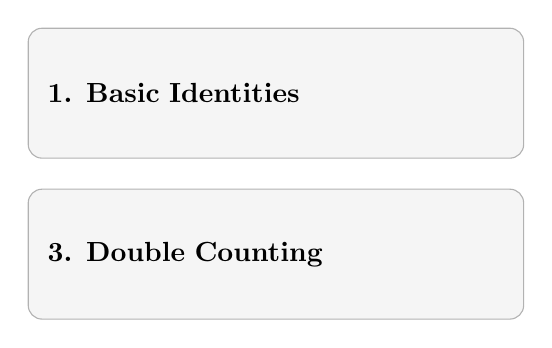
\begin{tikzpicture}\node[topic](a){\textbf{1. Basic Identities}};\node[topic,below=.38cm of a]{\textbf{3. Double Counting}};\end{tikzpicture}\end{column}\begin{column}{.48\textwidth}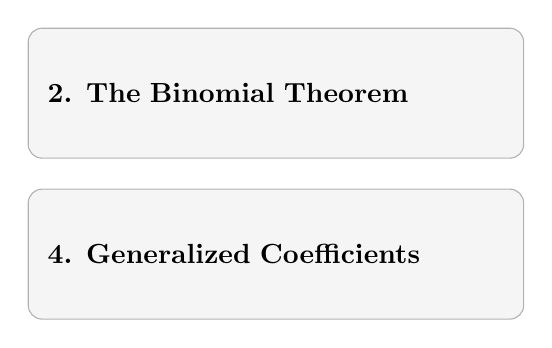
\begin{tikzpicture}\node[topic](a){\textbf{2. The Binomial Theorem}};\node[topic,below=.38cm of a]{\textbf{4. Generalized Coefficients}};\end{tikzpicture}\end{column}\end{columns}\end{frame}
\begin{frame}{One number, several interpretations}
\large
\[\binom nk\]
counts $k$-element subsets of an $n$-element set, binary words of length $n$ with $k$ ones, and lattice paths with $k$ up steps and $n-k$ right steps.
\gap Each interpretation suggests different identities.
\end{frame}
\begin{frame}{Conventions}
\large
\[\binom nk=\frac{n!}{k!(n-k)!}\qquad(0\leq k\leq n).\]
For nonnegative integer $n$, use
\[\binom nk=0\quad\text{if }k<0\text{ or }k>n.\]
\gap Also $\binom n0=\binom nn=1$, including $\binom00=1$.
\end{frame}
\begin{frame}{Symmetry}
\large
\Thm{Identity}{\[\binom nk=\binom n{n-k}.\]}
\Proof{Taking complements is a bijection from $k$-subsets to $(n-k)$-subsets of a fixed $n$-element set.}
\end{frame}
\begin{frame}{Pascal's identity}
\large
\Thm{Identity}{For $n\geq1$,
\[\binom nk=\binom{n-1}k+\binom{n-1}{k-1}.\]}
\Proof{Fix one element $a$. A $k$-subset either omits $a$, or contains $a$ and $k-1$ of the other elements. These two cases are disjoint.}
\end{frame}
\begin{frame}{Pascal's triangle}
\large
\begin{center}\renewcommand{\arraystretch}{1.25}
\begin{tabular}{c|rrrrrrr}
$n$&&&&&&&\\\hline
0&1\\1&1&1\\2&1&2&1\\3&1&3&3&1\\4&1&4&6&4&1\\5&1&5&10&10&5&1\\6&1&6&15&20&15&6&1
\end{tabular}\end{center}
Each interior entry is the sum of the two entries immediately above it.
\end{frame}
\begin{frame}{The binomial theorem}
\large
\Thm{Binomial theorem}{For every nonnegative integer $n$,
\[(x+y)^n=\sum_{k=0}^n\binom nk x^{n-k}y^k.\]}
\gap The coefficients of a familiar algebraic expansion count choices.
\end{frame}
\begin{frame}{A combinatorial proof}
\large
\Proof{Expand the product of $n$ factors $(x+y)$. To obtain $x^{n-k}y^k$, choose the $k$ factors that contribute $y$; all others contribute $x$.\gap There are $\binom nk$ such choices, which is exactly the coefficient of $x^{n-k}y^k$.}
\end{frame}
\begin{frame}{An example}
\large
\[(x+y)^5=x^5+5x^4y+10x^3y^2+10x^2y^3+5xy^4+y^5.\]
\Question{What is the coefficient of $x^3y^4$ in $(2x-y)^7$?}
\gap It is
\[\binom74 2^3(-1)^4=280.\]
\end{frame}
\begin{frame}{Row sums}
\large
\Thm{Identity}{\[\sum_{k=0}^n\binom nk=2^n.\]}
\Proof{Set $x=y=1$ in the binomial theorem. Alternatively, count all subsets by their sizes.}
\end{frame}
\begin{frame}{Alternating row sums}
\large
\Thm{Identity}{For $n\geq1$,
\[\sum_{k=0}^n(-1)^k\binom nk=0.\]}
\Proof{Set $x=1,y=-1$. A combinatorial proof pairs each subset with the subset obtained by toggling one fixed element. Each pair contains one even-sized and one odd-sized subset.}
\end{frame}
\begin{frame}{Even and odd subsets}
\large
\[\sum_{\substack{k=0\\k\text{ even}}}^n\binom nk
=\sum_{\substack{k=0\\k\text{ odd}}}^n\binom nk=2^{n-1}\qquad(n\geq1).\]
\gap Add and subtract the ordinary row sum and alternating row sum.
\end{frame}
\begin{frame}{A distinguished element}
\large
\Thm{Identity}{\[k\binom nk=n\binom{n-1}{k-1}.\]}
\Proof{Count pairs $(S,a)$ where $S$ is a $k$-subset and $a\in S$. Choose $S$ then $a$, or choose $a$ then the other $k-1$ elements of $S$.}
\end{frame}
\begin{frame}{A weighted row sum}
\large
\Thm{Identity}{For $n\geq1$,
\[\sum_{k=0}^n k\binom nk=n2^{n-1}.\]}
\Proof{Count a subset together with one distinguished member. Choose that member in $n$ ways, then choose any subset of the other $n-1$ elements.}
\end{frame}
\begin{frame}{Two distinguished elements}
\large
\Thm{Identity}{For $n\geq2$,
\[\sum_{k=0}^n k(k-1)\binom nk=n(n-1)2^{n-2}.\]}
\Proof{Count a subset with an ordered pair of distinct distinguished members. Choose those members first, then any subset of the remaining $n-2$ elements.}
\end{frame}
\begin{frame}{The sum involving $k^2$}
\large
Since $k^2=k(k-1)+k$, for $n\geq2$,
\[\sum_{k=0}^n k^2\binom nk=n(n-1)2^{n-2}+n2^{n-1}
=n(n+1)2^{n-2}.\]
\gap The identity for a more complicated weight follows from simpler counting interpretations.
\end{frame}
\begin{frame}{Vandermonde's identity}
\large
\Thm{Identity}{For nonnegative integers $r,s,m$,
\[\binom{r+s}{m}=\sum_{k=0}^m\binom rk\binom s{m-k}.\]}
\Proof{Split a set into parts of sizes $r$ and $s$. Count its $m$-subsets according to the number $k$ chosen from the first part.}
\end{frame}
\begin{frame}{Vandermonde by coefficients}
\large
\Proof{The identity
\[(1+x)^{r+s}=(1+x)^r(1+x)^s\]
gives two expressions for the coefficient of $x^m$. On the right, choose $x^k$ from the first factor and $x^{m-k}$ from the second, and sum over $k$.}
\gap This is our first example of a convolution of two sequences.
\end{frame}
\begin{frame}{A sum of squares}
\large
\Thm{Identity}{\[\sum_{k=0}^n\binom nk^2=\binom{2n}n.\]}
\Proof{Use Vandermonde with $r=s=m=n$ and symmetry:
\[\binom n{n-k}=\binom nk.\]}
\end{frame}
\begin{frame}{The hockey-stick identity}
\large
\Thm{Identity}{For $0\leq r\leq n$,
\[\sum_{j=r}^n\binom jr=\binom{n+1}{r+1}.\]}
\Proof{Count $(r+1)$-subsets of $\{1,\ldots,n+1\}$ according to their largest element $j+1$. The other $r$ elements can be chosen in $\binom jr$ ways.}
\end{frame}
\begin{frame}{Nested subsets}
\large
\Thm{Identity}{For $0\leq r\leq k\leq n$,
\[\binom nk\binom kr=\binom nr\binom{n-r}{k-r}.\]}
\Proof{Count pairs $R\subseteq K\subseteq[n]$ with $|R|=r$ and $|K|=k$. Choose the larger set first, or choose the smaller set first.}
\end{frame}
\begin{frame}{Generalized binomial coefficients}
\large
\Def{Definition}{For a number $x$ and a nonnegative integer $k$, define
\[\binom xk=\frac{x(x-1)\cdots(x-k+1)}{k!},\qquad\binom x0=1.\]}
\gap This is a polynomial in $x$. It need not count subsets when $x$ is not a nonnegative integer.
\end{frame}
\begin{frame}{Negative upper arguments}
\large
\Thm{Identity}{For positive integer $m$ and $k\geq0$,
\[\binom{-m}k=(-1)^k\binom{m+k-1}k.\]}
\Proof{Factor $-1$ from each of the $k$ numerator factors:
\[\frac{(-m)(-m-1)\cdots(-m-k+1)}{k!}
=(-1)^k\frac{m(m+1)\cdots(m+k-1)}{k!}.\]}
\end{frame}
\begin{frame}{Pascal's identity still holds}
\large
\Thm{Identity}{For $k\geq1$ and any $x$,
\[\binom xk=\binom{x-1}k+\binom{x-1}{k-1}.\]}
\Proof{Both sides are polynomials in $x$. They agree for all sufficiently large integers $x$ by Pascal's identity, and therefore agree identically.}
\end{frame}
\begin{frame}{A useful infinite expansion}
\large
\[(1-z)^{-m}=\sum_{k\geq0}\binom{m+k-1}kz^k\qquad(m\geq1).\]
\gap As a numerical series this holds for $|z|<1$. As a formal power series it is an identity of coefficients.
\gap We will recover these coefficients when counting selections with repetition.
\end{frame}
\begin{frame}{Practice}
\large
\Question{Prove
\[\sum_{k=r}^n\binom nk\binom kr=\binom nr2^{n-r}.\]}
\gap Count a subset $S\subseteq[n]$ together with a distinguished $r$-subset $R\subseteq S$.
\end{frame}
\begin{frame}{Practice: solution}
\large
\Proof{On the left, first choose $|S|=k$, then $S$, then $R$.\gap On the right, first choose $R$ in $\binom nr$ ways. Each of the remaining $n-r$ elements is independently either included in $S$ or excluded.\gap Both procedures count every pair $(R,S)$ exactly once.}
\end{frame}
\begin{frame}{Summary}
\large
\begin{itemize}
\item Binomial coefficients count subsets and appear as expansion coefficients.
\item Pascal, Vandermonde, and hockey-stick identities have direct counting proofs.
\item Distinguished elements produce weighted sums.
\item Generalized coefficients extend the algebra beyond nonnegative upper arguments.
\end{itemize}
\end{frame}
\begin{frame}{Next time: Multinomial Coefficients}\begin{center}{\Huge Multinomial Coefficients}\end{center}\end{frame}
\end{document}